\section{Численные эксперименты}

\indent
\indent
В данной главе мы обсудим экспериментальную часть работы, начиная от
архитектуры программы и заканчивая обсуждением полученных результатов.



\subsection{Архитектура программы}

\indent
\indent
Основная часть программы, выполняющая обучение и тестирование модели,
 состоит из стандартного для фреймворка \textit{pytorch} набора 
 взаимосвязанных компонент (классов). Перечислим их:

\begin{itemize}

	\item
	\textit{Module} --- описывает непосредственно вычислительный граф нейросети. 
	Здесь указаны параметры и количество всех слоев, описаны связи между ними.
	
	\item
	\textit{Dataset} --- позволяет итерироваться по набору данных и объединять 
	примеры в батчи для подачи на вход модели.
	
	\item
	\textit{Loss} --- вычисляет функцию ошибки (потери) между предсказанными 
	моделью  и правильными значениями целевой переменной.
	
	\item
	\textit{Optimizer} --- совершает шаг градиентого спуска на заданное расстояние,
	которое определяется скоростью обучения \textit{(learning rate)}. А именно,
	изменяет веса модели так, чтобы уменьшить среднюю ошибку для очередного
	переданного на вход модели батча данных.
	
	\item
	\textit{Scheduler} --- изменяет скорость обучения модели \textit{(learning rate)}
	с течением времени по заданному правилу.
	
	\item
	\textit{Stopper} --- останавливает тренировку при выполнении заданного 
	условия, например, если в течение последних \textit{n} эпох не произошло
	увеличения точности модели хотя бы на $\epsilon$.
	
	\item
	\textit{MetricsCalculator} --- оценивает точность модели на некоторой размеченной
	подвыборке данных по заданным метрикам.
	
	\item
	\textit{TensorboardX}  --- система для визуального логирования обучения
	модели в реальном времени;
	позволяет строить графики изменения функции ошибки, метрик и
	выводить любые другие пользовательские графики и изображения.
	
	\item
	\textit{Trainer} -- объединяет воедино компоненты, названные выше. Обучает
	модель эпоху за эпохой, с заданной частотой проверяет достигнутую точность
	на заранее определенном подмножестве данных. Останавливает тренировку по
	достижению некоторого критерия. Сохраняет промежуточные
	веса модели. Визуализирует процесс обучения.
 
 \end{itemize}


 \indent
 \indent
 Взаимосвязь между компонентами программы можно проследить на 
  рисунке \ref{tikzpicture: programm}.

\begin{figure}[h!]
    \begin{center}
   	    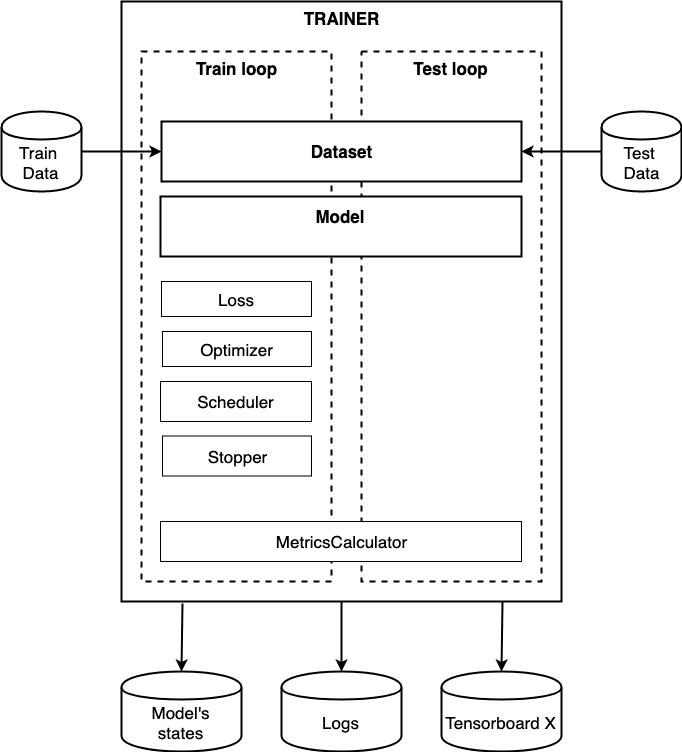
\includegraphics[width=0.95\linewidth]{Programm}
   	\end{center}
   	\caption{Структура программы для тренировки и обучения модели.}
   	\label{tikzpicture: programm}
\end{figure}


\subsection{Выбор метрики}

\indent
\indent
Прежде всего необходимо определиться, как количественно будет оцениваться
точность модели. Мы случайно выберем 80\% данных 
для тренировки моделей и 
20\% для их тестирования. В качестве метрик будем использовать 
классические для задачи классификации точность
 (\textit{accuracy}, не путать с \textit{precision}) и взвешенную (или
 сбалансированную по размерам классов) точность:
выражения \ref{eq:accuracy} и \ref{eq:w_accuracy}.


\begin{equation}\label{eq:accuracy}
	   acc(\vec{y^{gt}}, \vec{y}) = \frac{1}{N}\sum_{i=1}^{N} \delta_{y_i^{gt}, y_i}
\end{equation}
где $\vec{y^{gt}}$ --- вектор номеров классов длинной $N$, 
$\vec{y}$ --- вектор предсказанных номеров классов длинной $N$,
$N$ --- количество рассматриваемых примеров,
$\delta$ --- символ Кронекера.

\begin{equation}\label{eq:w_accuracy}
	   acc_w(\vec{y^{gt}}, \vec{y}) = 
	   \frac{1}{C} \sum_{c}
	   \frac{1}{N_c}\sum_{\{i: y_i^{gt}\equiv c\}} \delta_{y_i^{gt}, y_i}
\end{equation}
где $N_c$ --- количество примеров из класса $c$, $C$ --- количество классов.
 

\indent
\indent
Таким образом, чтобы посчитать точность, достаточно просто разделить
количество правильных ответов на общее количество ответов. Чтобы посчитать
взвешенную точность, необходимо вычислить точность для каждого класса
в отдельности, а затем усреднить полученные значения. В случае, если распределение
по классам в значительной степени неравномерное, отсутствие такого усреднения
приведет к тому, что значение метрики будет определяться точностью модели на
нескольких наиболее представленных классах. В данной работе мы будем
смотреть на значения обоих вариантов точности, но для принятия
решений о выборе модели приоритетной является взвешенная точность, так как в нашем наборе данных присутствует большой по размеру класс \textit{"другое"} (далее \textit{other}).


\subsection{Ход экспериментов}

\indent
\indent
Чтобы обучить модель оптимальным образом, сначала проведем серию
легковесных (с вычислительной точки зрения) экспериментов, чтобы определиться 
со значениями основных гиперпараметров. Затем попробуем улучшить целевую метрику
для лучшей модели, полученной на первом шаге.

\indent
\indent
Начнём с топологии нейронной сети. Будем выбирать из трех семейств архитектур:
\textit{ResNet}, \textit{Inception} и \textit{VGG};
их подробное описание приведено в разделе \ref{section:archs}.
Чтобы ускорить эксперименты уменьшим размер всех изображений до
$256 \times 256$ пикселей и не будем использовать аугментации во время тренировки.
Прекратим обучение после 50-ти
эпох\footnote{\textit{Эпохой} в машинном обучении называется один полный проход по
обучающему набору данных в процессе тренировки.}, либо остановимся досрочно,
если в течение 5-ти последних эпох не было улучшено 
значение метрики хотя бы на 0.5\%. В качестве функции потерь используем
 перекрестную энтропию (см. раздел \ref{section: losses}),
 а в качестве оптимизатора параметров 
нейронной сети --- \textit{Adam} \cite{adam}, т.к. он не требует тонкой настройки
параметров. Кроме того, отследим время, которое 
понадобилось на обучение модели до остановки эксперимента.
В качестве финального состояния модели выберем
то, которое соответствует моменту достижения максимального значения метрики
на тестовой выборке (это совсем не обязательно происходит на последней эпохе).


\begin{table}[h!]
    \begin{center}
        \begin{tabular}{c | c| c | c | c}
            \hline
            № & Архитектура & Точность & Взвешенная точность  & Время [мин] \\
            \hline
    
            1 & Inception v3 & 0.743 & 0.667 & 239 \\
            
            2 & VGG 11 & 0.678 & 0.565 & 154 \\
            
            3 & VGG 13 & 0.637 & 0.478 & 450 \\
            
            4 & ResNet 18 & 0.692 & 0.602 & 35 \\
            
            5 & ResNet 34 & 0.703 & 0.634 & 119 \\
            
            6 & ResNet 50 & 0.659 & 0.593 & 114 \\
    
            \hline
        \end{tabular}
    \end{center}
    \caption{Сравнение различных архитектур.}
    \label{tabular: arch_compare}
\end{table}


\indent
\indent
Как видно из результатов предварительных экспериментов
(таблица \ref{tabular: arch_compare}), наибольшую
точность показала архитектура \textit{Inception v3}. При этом 
\textit{ResNet34} уступает в точности незначительно, но требует
в 2 раза меньше времени на обучение, поэтому мы остановим свой
выбор на этой модели. 


Теперь попытаемся улучшить точность базовой модели,
используя различные техники тренировки и изменяя основные гиперпараметры.

\indent
\indent
\textbf{Оптимизатор}

\indent
Используем другой оптимизатор, например,
\textit{SGD}\footnote{Stochastic gradient descent (стохастический 
градиентный спуск)} с 
разными значениями скоростей обучения.
Кроме того, попробуем изменять скорость обучения в процессе тренировки:
будем её постепенно понижать и повышать.
Подразумевается, что такой подход может
помочь вывести функцию потерь из локального минимума. Данный
метод описан в статье 2017 года
\textit{Stochastic gradient descent with Warm Restarts}~\cite{cosine},
хотя его основная идея возникла ещё в 1983 году в публикации
\textit{Optimization by simulated annealing}~\cite{annealing}. В соответствии со
статьёй, скорость обучения изменяется по формуле \ref{eq:cosine}.

\begin{equation}\label{eq:cosine}
    lr_i = lr_{min} + \frac{1}{2} (lr_{max} - lr_{min}) (1 + \cos(\frac{i}{T} \pi ))
\end{equation}
где $lr$ -- скорость обучения,
$lr_{min}$ -- минимальная скорость обучения,
$lr_{max}$ -- максимальная скорость обучения,
$i$ -- номер текущей эпохи,
$T$ -- полупериод изменения скорости обучения. 

\indent
В настоящей работе использованы два набора параметров:
$lr_{min} = 0.001$, $lr_{max} = 0.1$ и $T = 3$ и
$lr_{min} = 0.001$, $lr_{max} = 0.1$ и $T = 50$. 
Напомним, что мы собираемся совершить не более 50-ти эпох.
В первом случае мы получаем так называемый косинусный отжиг,
так как скорость обучения то увеличивается, то уменьшается.
Второй набор параметров соответствует плавному
уменьшению скорости обучения в течение всей тренировки:
это может помочь быстро найти примерный регион,
где находится глобальный
минимум целевой функции, а затем уточнить его местоположение.
Соответствующие графики изменения
скорости обучения приведены на рисунке \ref{tikzpicture: cosine}.
Разумеется, понять,
какая из эвристик окажется лучшей в конкретном случае, позволит
только эксперимент.


\begin{figure}[h]
    \begin{center}
   	    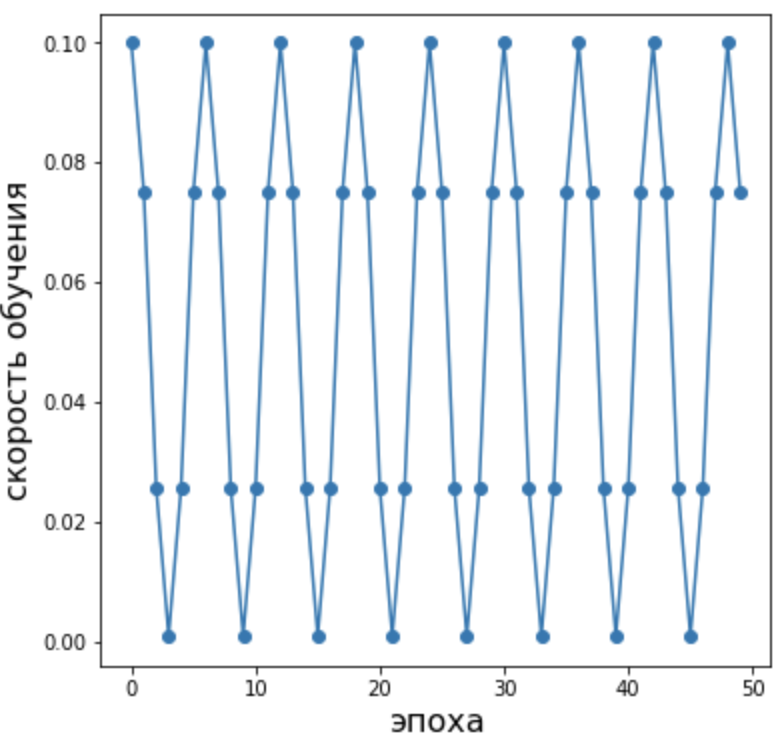
\includegraphics[width=0.5\linewidth]{cosine}
   	\end{center}
   	\caption{Изменение скорости обучения в процессе тренировки.}
   	\label{tikzpicture: cosine}
\end{figure}


\indent
\indent
\textbf{Размер изображений}

\indent
Попробуем уменьшать изображения не так сильно: 
до разрешения $512 \times 512$ вместо $256 \times 256 $.
С одной стороны, это сохранит больше информации, но с другой, увеличит 
количество пикселей в 4 раза, что уменьшит размер
батча и замедлит тренировку.
Поэтому необходимо соблюсти баланс между приростом точности,
которого можно добиться использованием изображений большего размера,
и увеличением времени тренировки.


\indent    
\indent
\textbf{Тренировочные аугментации}

\indent
Применим технику \textit{train time augmentations}, заключающуюся
в намеренном искажении данных, поступающих на вход модели.
Данный подход был описан ещё в 1977 году \cite{em_augs}, а термин 
\textit{augmentations} впервые возник в статье 1987 года \cite{augs}.
Использование случайных преобразований обрабатываемых
изображение позволяет искусственно
раздуть размер тренировочного набора данных, увеличить его 
вариативность, что, в свою очередь, помогает бороться с переобучением
%footnote
модели\footnote{Переобучением называется ситуация, когда модель
запомнила правильные ответы для примеров из тренировочной выборки,
но не приобрела обобщающую способность. Другими словами, это ситуация,
когда модель имеет хорошее значение метрики на тренировочном наборе,
но очень плохое на тестовом.}.
%footnote
Но возникает вопрос о силе применяемых искажений.
Если трансформации слишком слабы, модель быстро адаптируется
 и её обобщающая 
способность не будет улучшена. Если слишком сильны, то визуальные паттерны, по
которым можно было бы классифицировать изображение, исчезнут. 
Кроме того, чтобы было удобно подбирать подходящую степень искажений,
необходимо каким-то образом количественно её охарактеризовать.
Поступим следующим образом:
для каждого применяемого преобразования выберем некоторое базовое значение 
параметра, соответствующее преобразованию средней силы. 
Затем, одновременно для всех преобразований, будем изменять значения параметров,
в $k$ раз увеличивая или уменьшая выбранные базовые значения.
Таким образом, при $k = 1$ используются трансформации 
с базовыми значениями параметров, при $k = 2$ с удвоенными 
значениями параметров и так далее. Кроме того, вероятность применить то или
иное преобразование так же задаётся параметрически:
$p = 0.4 + 0.1k$.
Перечислим используемые трансформации
и формулы для вычисления их параметров:

\begin{itemize}

    \item Поворот на угол от $-10k$ до $+10k$ градусов.

    \item Из изображения вырезается прямоугольник, линейный размер
    которого выбирается от $1 - 0.1k$ до $1$ размера изображения.
    
    \item Перенос на величину от $0$ до $0.1k$ от линейного
    размера изображения (по вертикали и горизонтали).
    
    \item Сдвиг на величину от $0$ до $0.05k$ от линейного
    размера изображения
    (по вертикали и горизонтали).
    
    \item Изменение отношения сторон в $s$ раз, где $s$ меняется
    от $1 - 0.1k$ до $1 + 0.1k$ от размера изображения.
    Причем большей стороной может оказаться как высота,
    так и ширина изображения.
    
    \item Случайное зеркальное отражение с вероятностью $p$
    (только по горизонтали).
    
    \item Изменения яркости, контраста, оттенка и насыщенности.
    Степень изменения задаётся числом от
    $max(0, 1 - 0.1k)$ до $1 + 0.1k$. Чем дальше это число отстоит от
    $1$, тем значительнее изменения.
    
\end{itemize}
    
    
\indent
\indent
\textbf{Тестовые аугментации}

\indent
Применим технику \textit{test time augmentations}.
Её смысл заключается в том, что на стадии использования модели
входное изображение
несколько раз копируется, и к копиям применяются различные 
искажения из числа тех, которые использовались во время тренировки.
После чего модель производит предсказание для каждой
копии, а в качестве окончательного ответа вычисляется, например, 
среднее значение по всем выходам модели. Для многих задач таким образом
удаётся улучшить точность предсказаний,
но сложность вычислений линейно возрастает
с количеством созданных копий.
В данной работе изображение копируется 8 раз.


\bigbreak
\indent
\indent
Используем техники, описанные выше, и проведём вторую серию 
экспериментов, направленных на усовершенствование
 выбранной ранее модели --
\textit{ResNet34}. Но на этот раз изменим критерий остановки: если раньше мы 
прекращали тренировку, когда значение метрики не увеличивалось хотя бы 
на 0.5\% за последние 5 эпох, то теперь будем ждать 15 эпох. Это связано
с тем, что для обучения с использованием аугментаций необходимо
больше времени для сходимости; мы так же будем
проводить эксперименты с уменьшенной
скоростью обучения, что тоже требует дополнительного времени.
Кроме того, уменьшим максимальное количество эпох для экспериментов
с разрешением $512 \times 512$ с 50-ти до 30-ти, так одна эпоха 
для изображений такого размера занимает слишком много времени.
Полученные результаты приведены в таблице \ref{tabular: train_tricks}.


\begin{table}[h!]
    \begin{center}
        \begin{tabular}{c | c| c | c | c| c| c}
            \hline
           № & Оптимизатор & Степень & Разрешение & Точность & Взвешенная  & Время \\
            & & аугментаций ($k$) & & & точность & [мин] \\
           \hline
    
           1 & Adam lr: 0.01 & 1 & $256 \times 256$ & 0.756 & 0.682 & 232 \\
           
           2 & SGD, lr: 0.01 & 1 & $256 \times 256$ & 0.800 & 0.739 & 320 \\
           
           3 & SGD, lr: 0.1 & 1 & $256 \times 256$ & 0.802 & 0.739 & 412 \\
           
           4 & SGD, lr: 0.01 & 3 & $256 \times 256$ & 0.815 & 0.747 & 302 \\
           
           5 & SGD, lr: 0.01 & 5 & $256 \times 256$ & 0.771 & 0.695 & 369 \\
           
           \hline
           6 & SGD, annealing & 1 & $256 \times 256$ & 0.8113 & 0.752 & 275 \\
            &  $T=3, lr_{max} = 0.1$ & & & & \\
           \hline
            
           7 & Adam lr: 0.001 & 2 & $256 \times 256$ & 0.745 & 0.688 & 266 \\
            
           8 & SGD, lr: 0.01 & 1 & $512 \times 512$ & 0.810 & \textbf{0.781} & 698 \\
           
           \hline
           9 & SGD, annealing & 2 & $512 \times 512$ & 0.830 & 0.766 & 867 \\
            &  $T=3, lr_{max} = 0.1$ & & & & \\
           \hline
           
           10 & SGD, annealing & 2 & $512 \times 512$ & 0.818 & 0.762 & 889 \\
            &  $T=50, lr_{max} = 0.1$ & & & & \\
           \hline
           
           11 & SGD, lr: 0.01 & 2 & $512 \times 512$ & 0.820 & 0.764 & 813 \\
           
            \hline
        \end{tabular}
    \end{center}
    \caption{Улучшение точности базовой модели (\textit{ResNet34}).}
    \label{tabular: train_tricks}
\end{table}


\indent
\indent
Как видно из результатов второй серии экспериментов, лучшая модель
была натренирована на изображениях разрешения
$512 \times 512$; использовался
оптимизатор SGD с постоянной скоростью обучения $lr: 0.01$ и применялись
аугментации средней силы. Точность достигла значения $0.810$, а
взвешенная точность -- $0.781$ (таблица \ref{tabular: train_tricks}, №8).
Эту модель мы будем использовать для дальнейшего исследования.
Отметим, что тренируясь на изображениях размера $256 \times 256$ и 
используя косинусный отжиг, нам удалось добиться почти такой же точности,
затратив в три раза меньше времени (таблица \ref{tabular: train_tricks}, №6).


\indent
\indent
По завершении тренировки было сделано ещё одно предсказание классов
для тестовой выборки с использованием описанной выше техники
\textit{test time augmentations}. Это позволило незначительно увеличить
точность: примерно на 0.01.


\subsection{Исследование модели}


\indent
\indent
Итак, нам удалось улучшить базовый
вариант тренировки модели \textit{ResNet34},
увеличив значение взвешенной точности на $0.147$ -- 
 c $0.634$ до $0.781$ (таблица \ref{tabular: train_tricks}, №8), 
при этом продолжительность 
тренировки выросла на порядок.


\indent
\indent
Теперь попробуем понять, в каких случаях и почему
 ошибается модель. Построим матрицу ошибок
 для тестового подмножества данных
(рисунок \ref{tikzpicture: conf_mat}),
чтобы увидеть,  как распределены неправильные
предсказания по различным классам (тегам).


\begin{figure}[h!]
    \begin{center}
   	    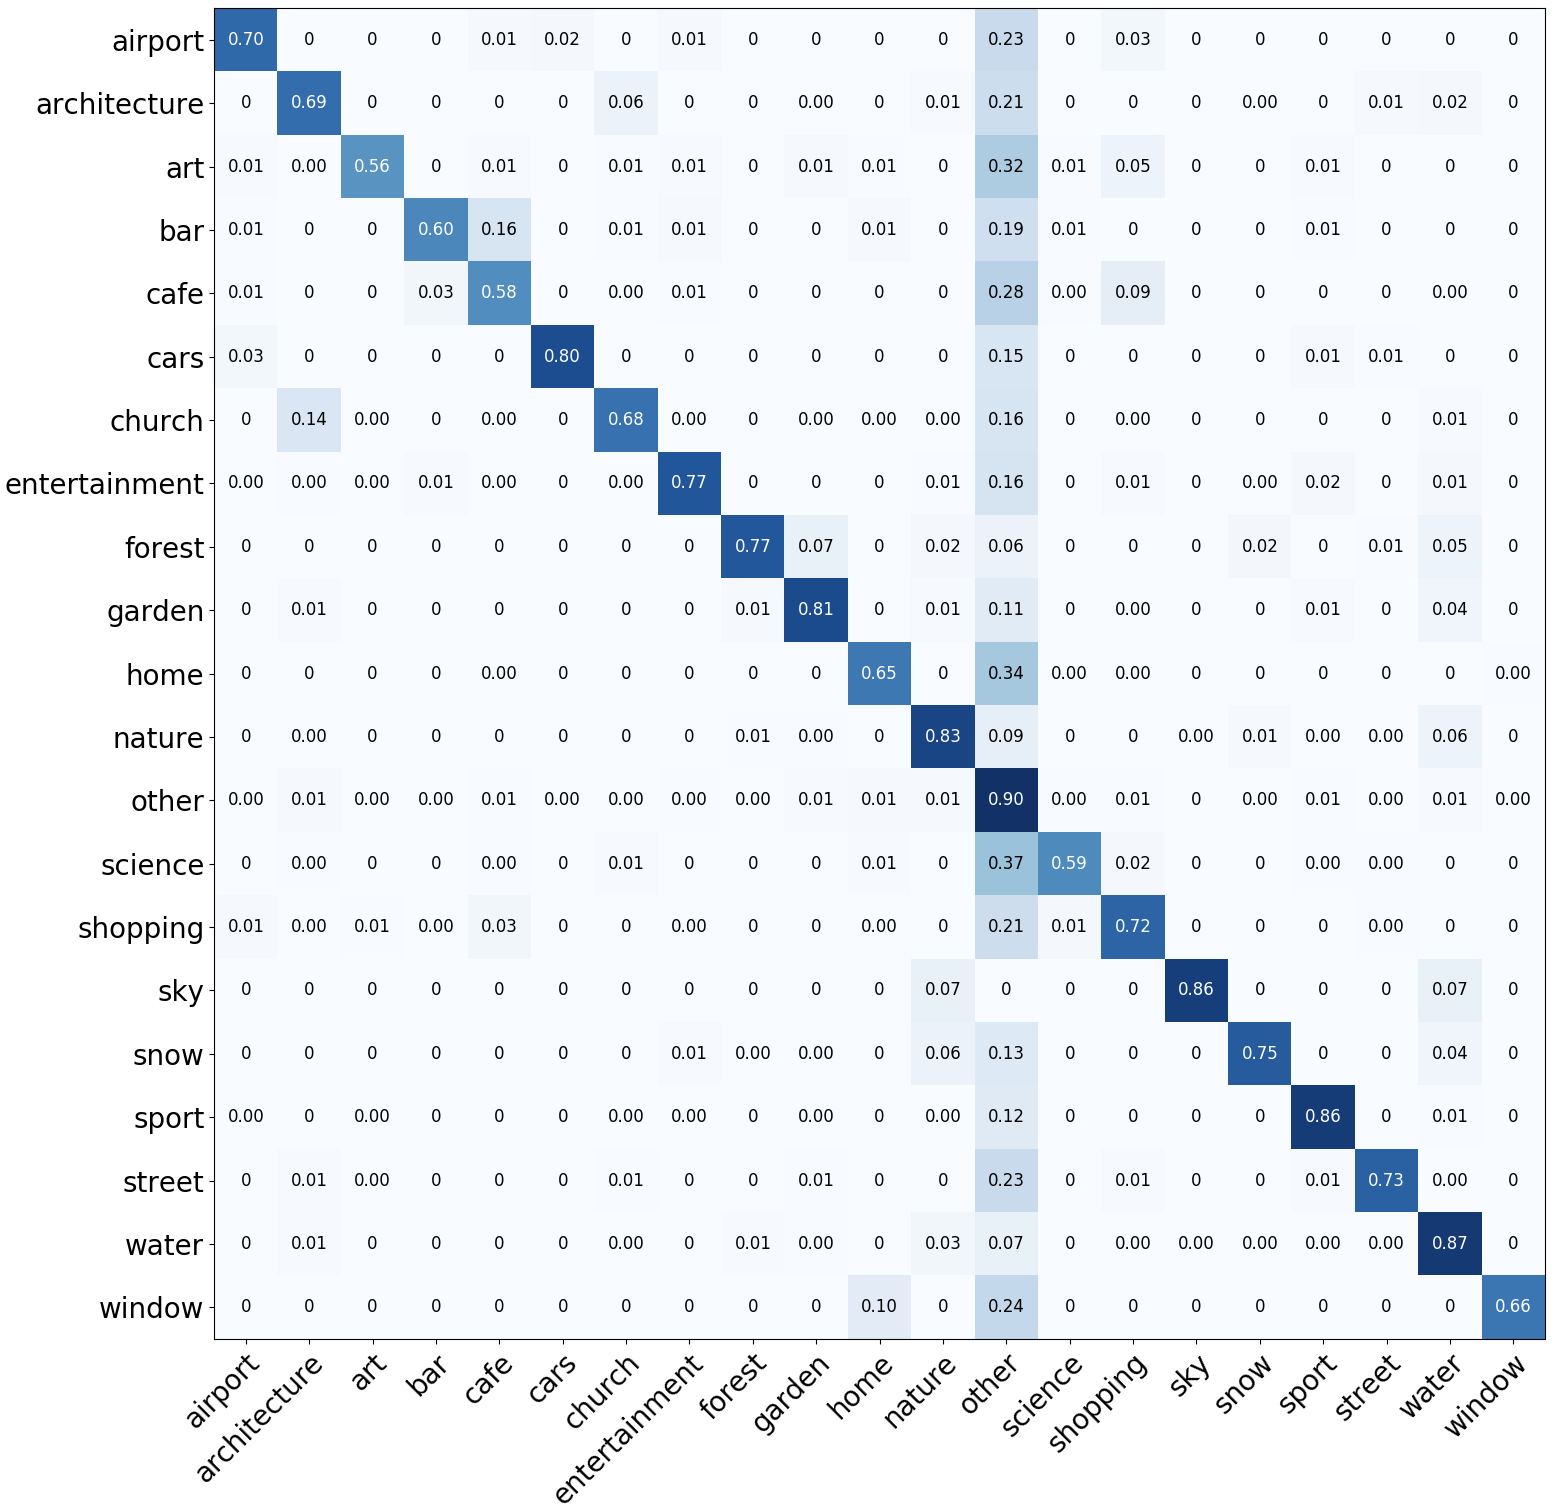
\includegraphics[width=0.98\linewidth]{conf_mat}
   	\end{center}
   	\caption{Матрица ошибок (\textit{confusion matrix}). Истинные метки 
   	               классов отложены по горизонтали, предсказанные -- по вертикали.}
   	\label{tikzpicture: conf_mat}
\end{figure}


\indent
\indent
Проанализируем матрицу ошибок.
Во-первых, её главная диагональ ярко выражена, что хорошо.
Во-вторых, предсказания класса \textit{other},
занимающего половину всего датасета, часто оказываются не 
точны (тёмная вертикальная полоса на рисунке \ref{tikzpicture: conf_mat}).
Это ожидаемое явление и оно не представляет большой проблемы, так как
мы просто не предложим пользователю какой-то хэштег, хотя могли бы.
Было бы хуже, если бы мы предлагали хэштег в случаях, где его 
быть не должно (такая ситуация соответствовала бы тёмной горизонтальной 
полосе на изображении матрицы ошибок).
В-третьих, можно заметить, что путаются похожие классы, 
некоторые представители
которых могут быть отнесены к нескольким классам одновременно.
Например, \textit{church} и \textit{architecture}; \textit{bar} и \textit{cafe};
\textit{nature} и \textit{water}.


\indent
\indent
Наконец, посмотрим, какие теги предсказала модель для конкретных
примеров из тестовой выборки. Корректные предсказания изображены
на рисунке \ref{tikzpicture: correct_predict}, а неправильные -- на
\ref{tikzpicture: err_predict}. Отобраны примеры, для которых сеть сделала
предсказания с наибольшим значением уверенности.
На рисунке \ref{tikzpicture: err_predict} видна
проблема для классов, упомянутых выше: модель ошибается на примерах, 
которые могли бы быть отнесены сразу к нескольким классам.


\indent
\indent
Дополнительно приведем скорость работы модели: на описанной ранее
конфигурации аппаратного обеспечения за 1 секунду производится
75 предсказаний для изображений размером $512 \times 512$.



\begin{figure}
    \begin{center}
   	    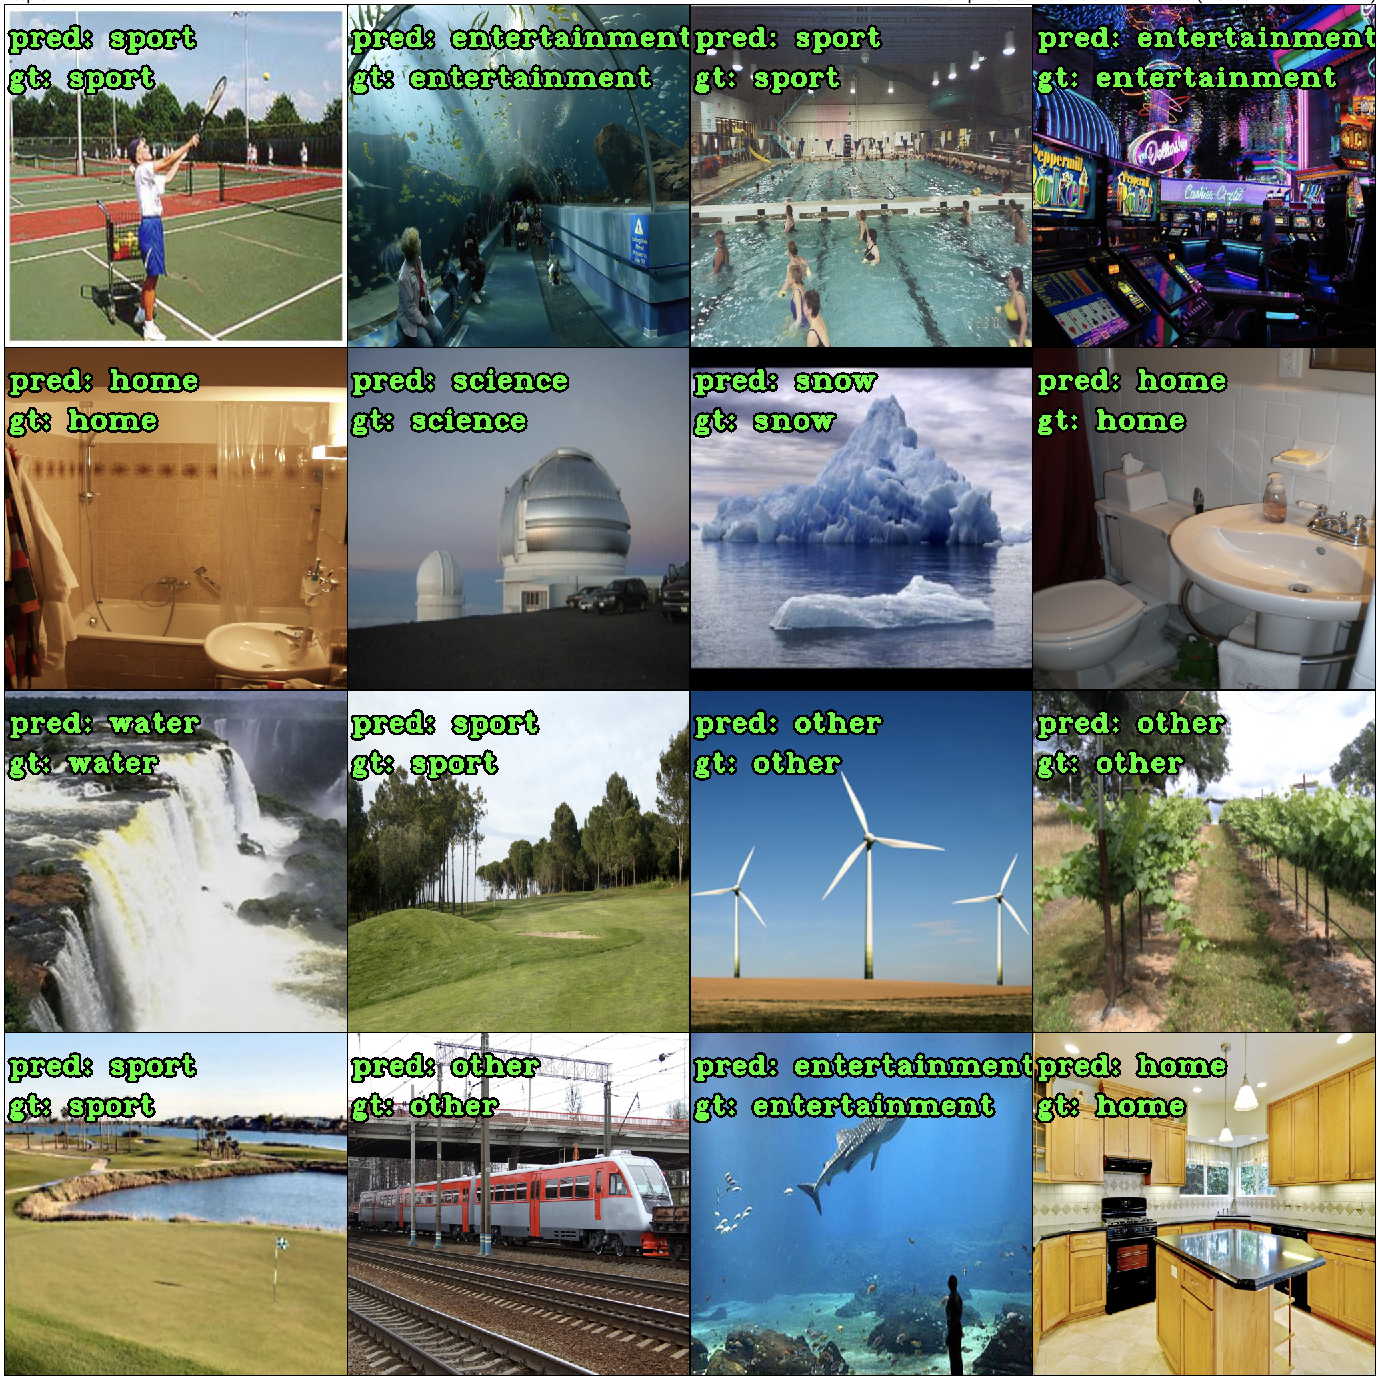
\includegraphics[width=0.9\linewidth]{correct_predict}
   	\end{center}
   	\caption{Примеры, для которых предсказанные
   	 \textit{(predicted)} и истинные \textit{(ground truth)} классы совпадают.}
   	\label{tikzpicture: correct_predict}
\end{figure}


\begin{figure}
    \begin{center}
   	    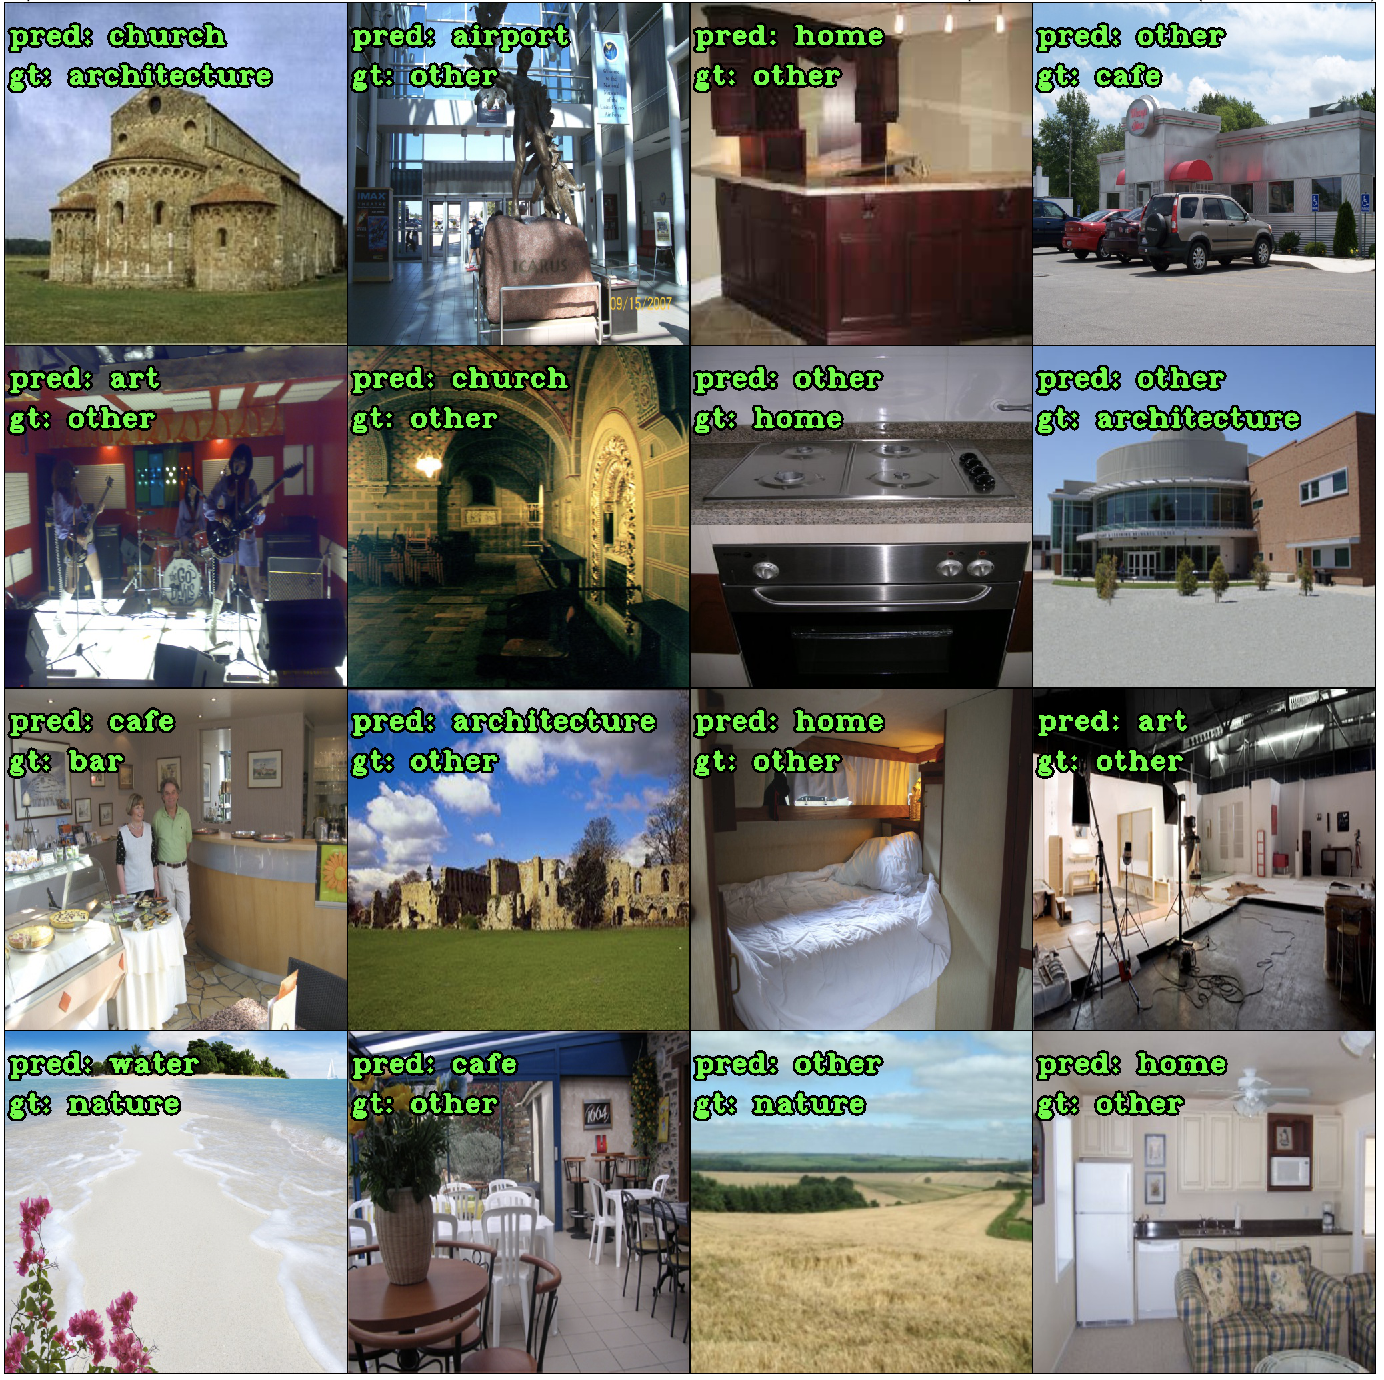
\includegraphics[width=0.9\linewidth]{err_predict}
   	\end{center}
   	\caption{Примеры, для которых предсказанные
   	 \textit{(predicted)} и истинные \textit{(ground truth)} классы не совпадают.}
   	\label{tikzpicture: err_predict}
\end{figure}
